\mode*

\section{Formattera strängar}

\subsection{Dokumentation}

\begin{frame}
  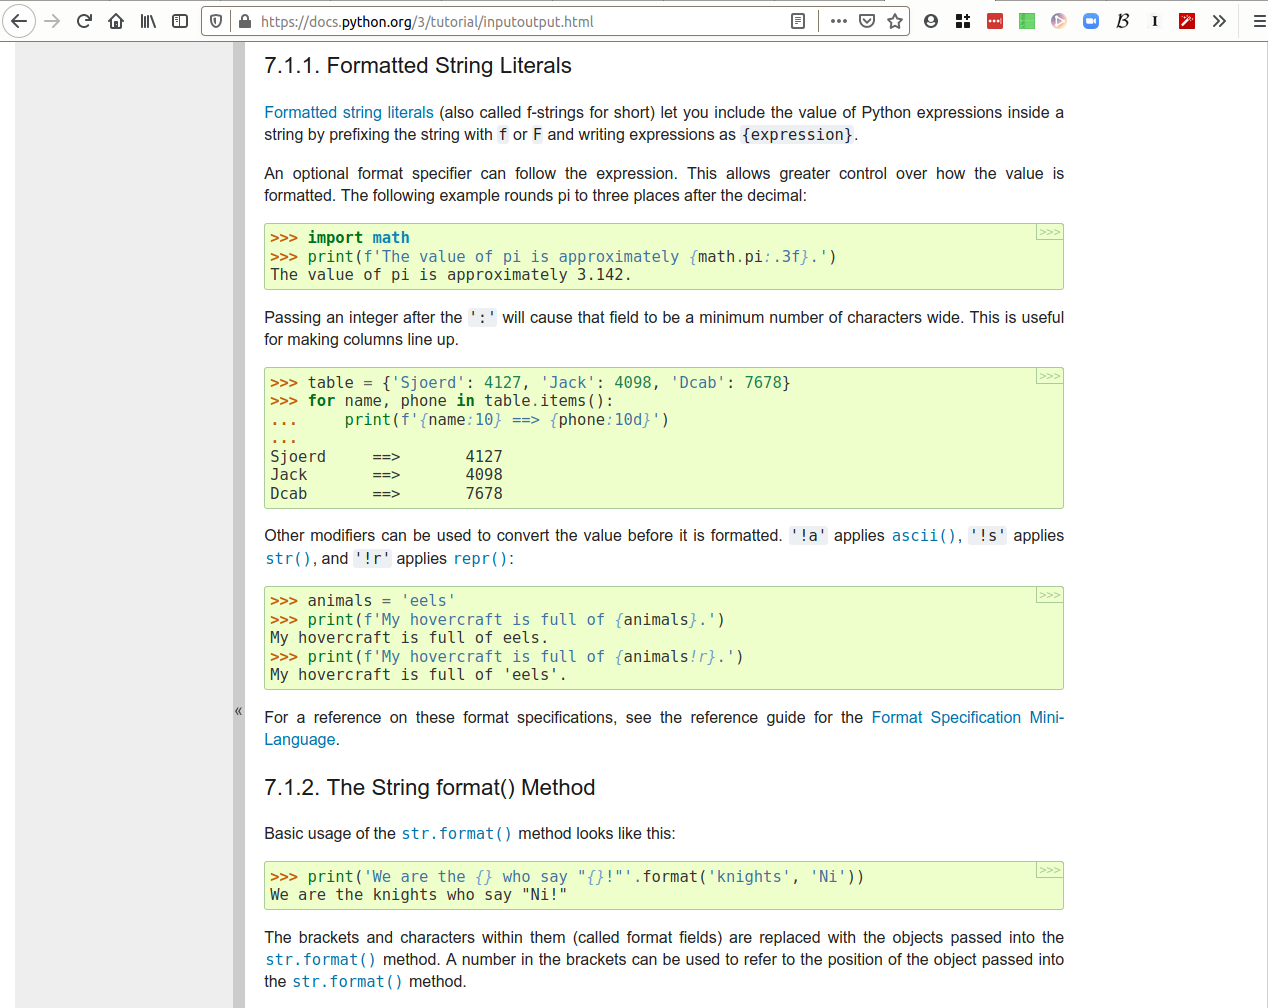
\includegraphics[width=\columnwidth]{figs/docs-strings.png}
\end{frame}


\subsection{Några fler saker man kan göra}

\begin{frame}
  \begin{example}[formatpi.py]
    \lstinputlisting{examples-more/formatpi.py}
  \end{example}
\end{frame}

\begin{frame}
  \begin{example}[align.py]
    \lstinputlisting{examples-more/align.py}
  \end{example}
\end{frame}

\begin{frame}
  \begin{example}[align-binary.py]
    \lstinputlisting{examples-more/align-binary.py}
  \end{example}
\end{frame}

